\section{Filter in der Bildverarbeitung} \label{sec:filter}

Das Ziel in der Bildverarbeitung ist meist die Extraktion von Informaionen bzw. die Erkennung von Objekten. In unserem Fall gilt es hauptsächlich herauszufinden, wo sich Linien im Bild befinden, die zur Fahrspur gehören. Hierbei kann das Graustufenbild als Matrix verstanden werden, deren Einträge die Helligkeit der einzelnen Pixel darstellen. Um bestimmte Eigenschaften zu ändern oder Informationen in einem Bild hervorzuheben, werden mathematische Operationen auf die Pixelmatrix angewendet. Diese Verfahren, deren Ergebnisse wieder ein Bild sind, teilen sich in Punktoperationen, Nachbarschaftsoperationen und globale Operationen auf \autocite{jaehneDigitaleBildverarbeitungMit2005}. Da Punktoperationen für jedes Pixel den Farb- oder Helligkeitswert neu berechnen, verwendet man sie typischerweise zur Korrektur von Kontrast, Helligkeit oder Farbraum. Objekte, wie zum Beispiel eine Straßenmarkierung, zeichnen sich meist dadurch aus, dass sich Pixel in Merkmalen von ihren Nachbarpixeln unterscheiden. Bei den Nachbarschaftsoperationen berechnen sich die Werte der Pixel des neuen Bildes aus den Bildpunkten einer kleinen Umgebung um die Punkte. Weil durch eine Nutzung des Nachbarschaftsoperators das Bild verändert wird und Informationen generell verloren gehen, spricht man auch von einem \emph{Filter}. Das von uns verwendete und sehr verbreitete Faltungsfilter verrechnet zur Ergebnisbildung die Helligkeitswerte über einen Filterkern miteinander. Der Filterkern ist hierbei eine quadratische, symetrische Matrix, die mit der Pixelmatrix des Bildes gefaltet wird. Die Faltung zweier Funktionen beschreibt die Gewichtung einer zeitabhängigen Funktion mit einer anderen. Unter dem Faltungsprodukt \( f_1(\gls{lat:time}) \ast f_2(\gls{lat:time}) \) zweier Originalfunktionen \(f_1(\gls{lat:time}) \) und \(f_2(\gls{lat:time}) \) versteht man allgemein das Integral \autocite{papulaMathematikFuerIngenieure}

% allgemeine Faltungsformel
\begin{equation}
f_1(\gls{lat:time}) \ast f_2(\gls{lat:time}) = \int \limits_{-\infty}^{+\infty} f_1(\gls{gre:laufvar_faltung}) \cdot f_2(\gls{lat:time}-\gls{gre:laufvar_faltung})d\gls{gre:laufvar_faltung}
\end{equation}

 Die Bildmatrix und der Filterkern sind aber diskret. Deswegen wird das Integral zu einer Summe. Seien \gls{lat:BildmatrixGefiltert} das gefilterte und \gls{lat:BildmatrixOriginal} das originale Bild, \gls{lat:Filterkernmatrix} der Filterkern, \(m\) und \(n\) dessen Matrixdimensionen und \( (a,b) \) der Mittelpunkt des Filterkerns, dann ergibt sich folgende Berechnungsformel für die diskrete Faltung:

% Formel diskrete Faltung:
\begin{equation}
\gls{lat:BildmatrixGefiltert}(x,y) = \sum_{i=1}^{m} \sum_{j=1}^{n} \gls{lat:BildmatrixOriginal}(x-i+a, y-j+b) \cdot \gls{lat:Filterkernmatrix}(i,j)
\end{equation}

Ein Faltungsfilter berechnet also den Wert des neuen Pixels aus dem gewichteten Mittelwert der umliegenden Pixel innerhalb des Filterkerns. Je nachdem, nach welcher Funktion gewichtet wird, ergibt sich der Name des Filters und was er in dem Bild bewirkt. 
%In dieser Arbeit wurden das Gauß-Filter zum Glätten und das Laplace-Filter zur Kanten- und letztlich Liniendetektion genutzt.

Eine gute Möglichkeit, Rechenzeit mit einem zweidimensionalen Filter einzusparen, ist, ihn so in zwei eindimensionale Operatoren zu zerlegen, dass deren Matrixmultiplikation wieder den ursprünglichen 2D-Filter ergibt. Wenn dies möglich ist, nennt man das Filter \emph{separierbar}. Die Anwendung des zweiten Operators auf das Zwischenergebnis des ersten auf das Bild hat das gleiche Ergebnis zur Folge, aber einen geringeren Rechenaufwand.

\subsection{Gauß-Filter}

Der Filterkern des Gauß-Filters stellt sich aus der diskretisierten Gaußfunktion auf. Dieses Filter ist ein Tiefpassfilter und wird zur Glättung und zum Weichzeichnen verwendet. Das Bildrauschen kann mit diesem Filter vermindert werden. Die diskrete Impulsantwort in zwei Dimensionen ergibt sich, wenn man die beiden Richtungen in \( x\) und \( y \) multipliziert.

% Formel für Gauß-Funktion (Impulsantwort bei zwei Dimensionen)
\begin{equation}
h(x,y) = \frac{1}{2\pi\sigma^2} \cdot e^{-\frac{x^2+y^2}{2\sigma^2}}
%\label{eq:gaussfkt}
\end{equation}

Mit dem Zusammenspiel von der Filterkerngröße und der Standartabweichung \( \sigma \) lässt sich einstellen, wie stark das Bild verwäscht. Je größer der Kern und \( \sigma \) ist, desto verschwommener ist das Resultat. In Abbildung~\ref{fig:grundlagen_gaussfilter} ist beispielhaft ein \( 15\times15\) - Filterkern mit \( \sigma = 3\) dargestellt.

\begin{figure}[H] % [htb]
  \centering
  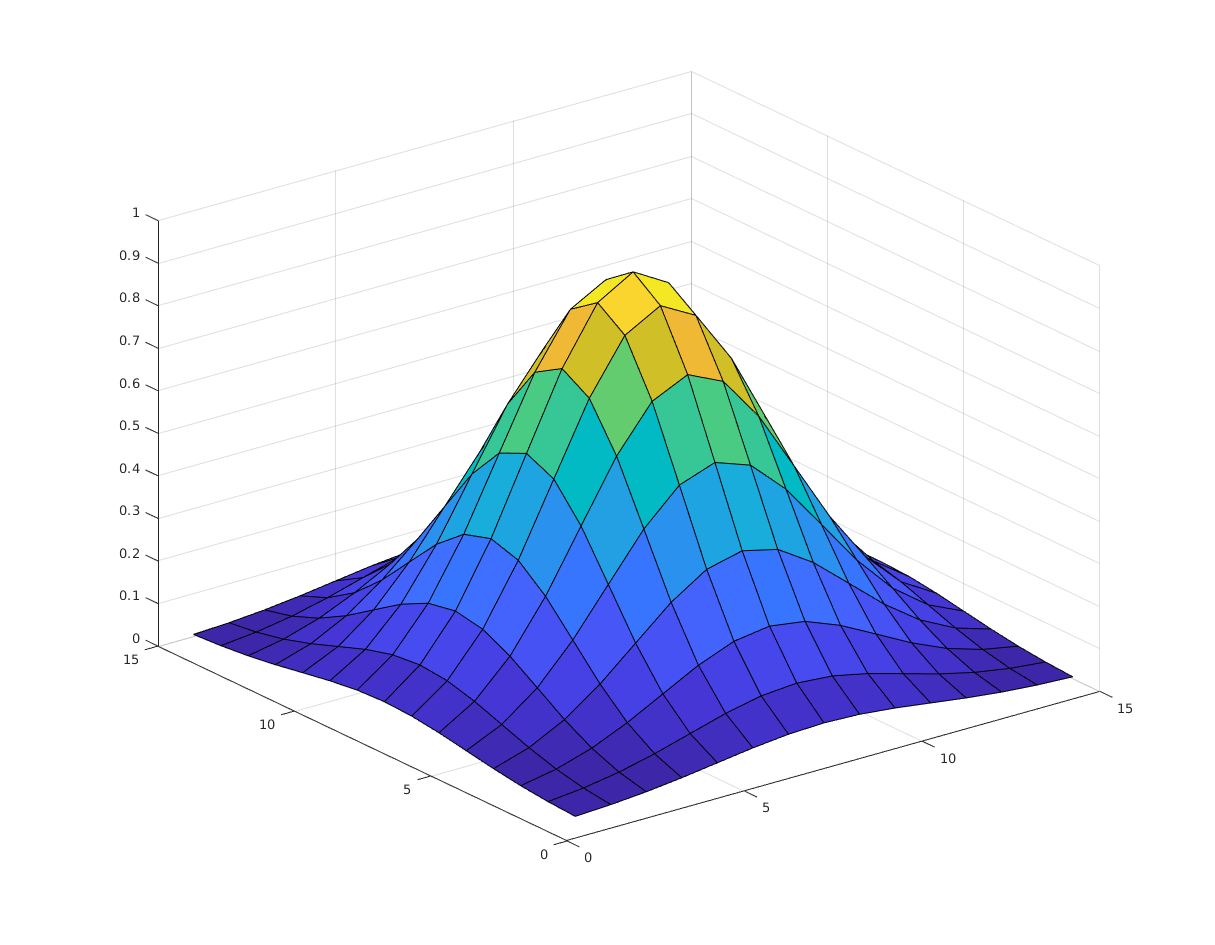
\includegraphics[width=0.9\textwidth]{grundlagen_gaussfilter.png}
  \caption{3D-Plot der Matrix eines \( 15\times15\) - Gauß-Filters}
  \label{fig:grundlagen_gaussfilter}
\end{figure}  

\subsection{Laplace-Filter}
% welcher starke Veränderungen in den Helligkeitsunterschieden zu benachbarten Pixeln hervorhebt.
%In der zweiten Ableitung sind Kanten die Nulldurchgänge 

Wenn man in einem Bild Kanten detektieren möchte, fundiert die Lösung des Problems immer auf Ableitungen in der einen oder anderen Form. (In der ersten Ableitung sind Kanten z.B. die Extremstellen.) Ein Filter zur Kantendetektion sollte Diskontinuitäten in den Grauwerten hervorheben und konstante Grauwerte unterdrücken. Der Laplace-Filter, bzw. diskrete Laplace-Operator, nutzt dafür die Summe der partiellen zweiten Ableitungen in alle Richtungen. \autocite{jaehneDigitaleBildverarbeitungMit2005}

% Formel für den Laplace-Operator
\begin{equation}
\Delta f = \frac{\partial^2 f}{\partial x^2} + \frac{\partial^2 f}{\partial y^2}
\end{equation}

% Die gesuchten Kanten sind dann die Nulldurchgänge in der zweiten Ableitung, vor und nach denen es unmittelbar Signalspitzen gibt, die höher als das Rauschen sind. 
Die Nulldurchgänge, vor und nach denen es unmittelbar Signalspitzen gibt, sind dann die gesuchten Kanten. Ein großer Nachteil dieser Filtermethode ist das relativ stark verrauschte Ergebnisbild.

Eine spezielle Form eines diskreten Laplace-Filters ist der \gls{acr:log}, welcher in dieser Arbeit zur Liniendetektion genutzt wurde. Der in Abbildung~\ref{fig:grundlagen_logfilter} beispielhaft dargestellte Filterkern wird durch die Anwendung des Laplace-Operators auf eine Gaußfunktion erstellt. Dieses Filter bewirkt neben der Kantendetektion eine gauß'sche Glättung und mindert so das störende Rauschen.

\begin{figure}[H] % [htb]
  \centering
  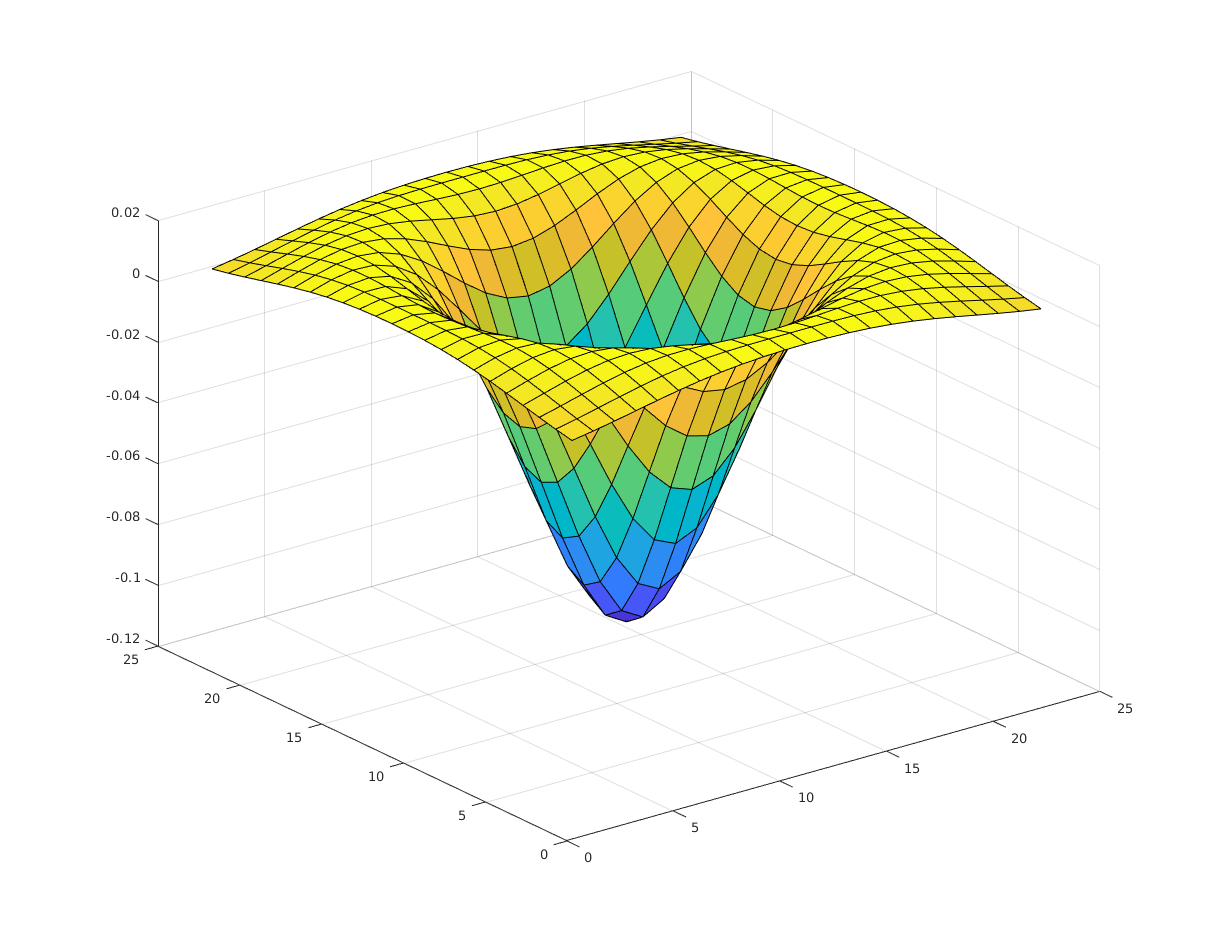
\includegraphics[width=0.9\textwidth]{grundlagen_logfilter.png}
  \caption{3D-Plot der Matrix eines \( 23\times23\) - \gls{acr:log}-Filters}
  \label{fig:grundlagen_logfilter}
\end{figure}  

